\vspace*{-5mm}
\mysection{Architectural Design}

\mysubsection{Overview}
In this chapter we will analyze the proposed architecture and components of the Travlendar+ system.\par
The proposed architecture has three tiers :
\begin{itemize}
	\setlength{\leftskip}{0.5cm}
	\item \emph{Presentation Tier : }represented by Browser and Mobile App. It's how the system shows himself to the user.
	\item \emph{Web and Business Tier : }represented by Web Server, which contains javascript and html code in order to create dynamic pages, and Application Server, which contains all the system's logic (the so called Business Logic).
	\item \emph{Database Tier : }represented by DB Server, that contains and manages persistent data in an efficient way.
\end{itemize}
\begin{figure}[H]
	\centering
	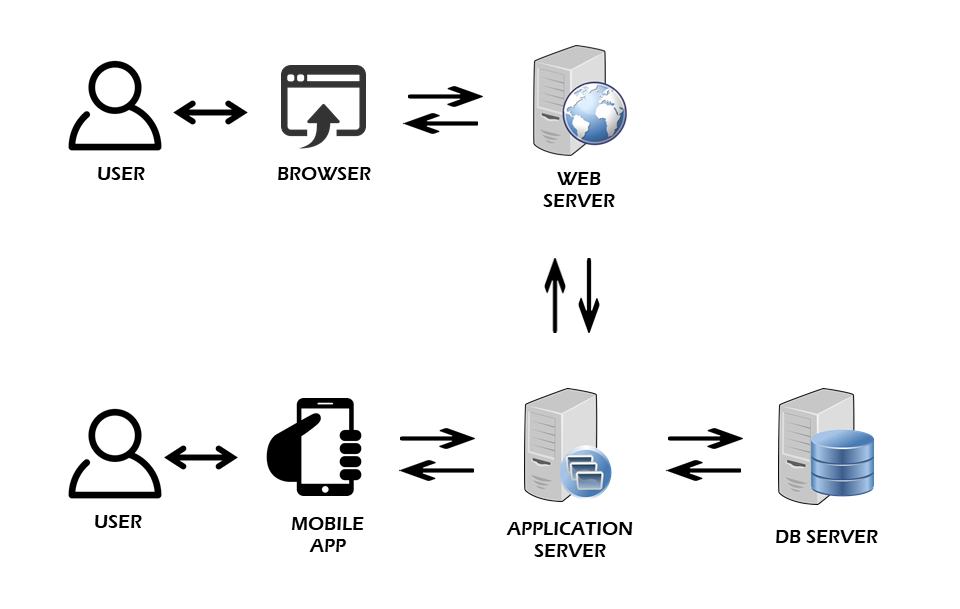
\includegraphics[scale=0.4]{Images/Architecture/Proposed_Architecture}
	\caption{Proposed Architecture}
\end{figure}

\mysubsection{High Level Components and Their Interactions}
Here we have a proposed High Level Component Diagram
\begin{figure}[H]
	\centering
	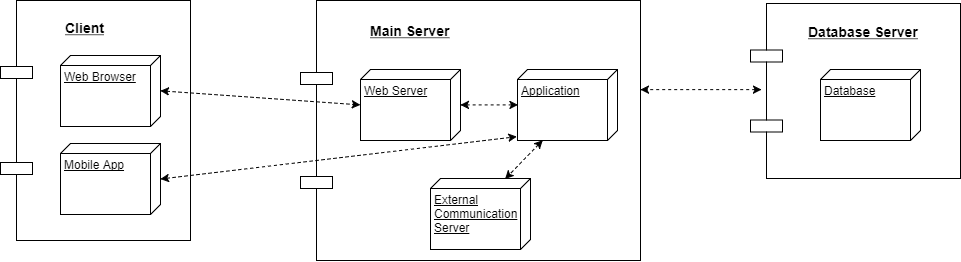
\includegraphics[scale=0.4]{Images/Architecture/Components_High_Level}
	\caption{Components High Level}
\end{figure}

Analyzing this Diagram we can see :
\begin{itemize}
	\setlength{\leftskip}{0.5cm}
	\item \emph{On the Client Side : }The Mobile App of Travlendar+ for all users that uses a smartphone and has already downloaded it or the Web Browser for all the others.
	\item \emph{On the Server Side : }The Web Server that, as told before, creates dynamic html and js pages, for the Web Browser, using data elaborated by the server's logic and the Application that is actually the server's logic. There is also a third component, the External Communication Server, that manages the communication of our server with the external ones, such as Google servers or Transport Service servers, in order to send and recieve informations and data from them.
	\item \emph{On the Database Side : }The Database used to contain and manage all data and informations that our system needs to handle.
\end{itemize}

\mysubsection{Component View}

TEXT HERE

\begin{figure}[H]
	\centering
	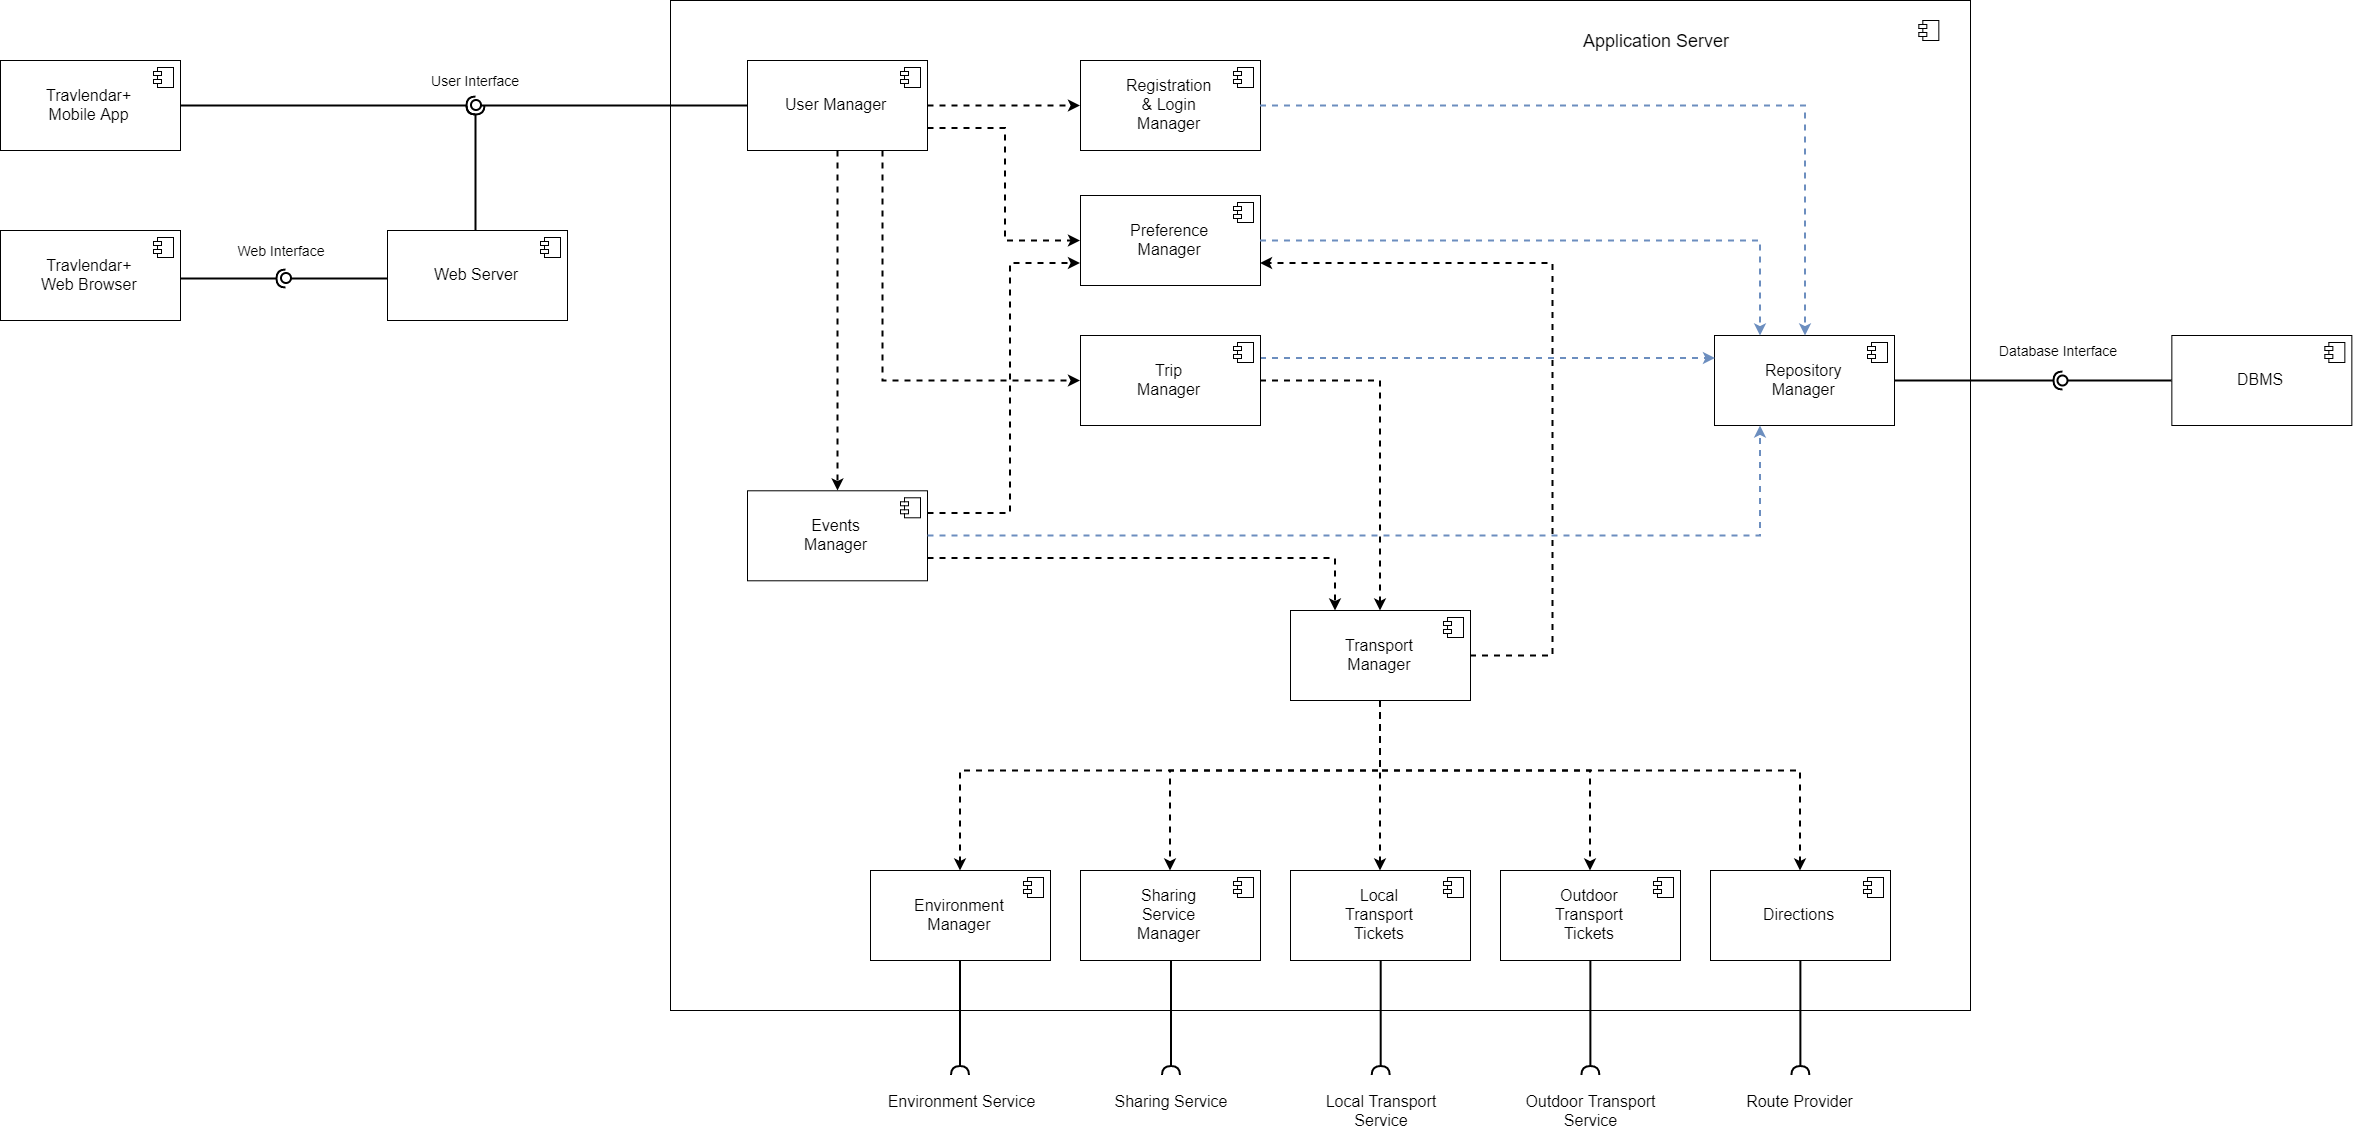
\includegraphics[scale=0.2]{Images/Architecture/Components_View}
	\caption{Component View}
\end{figure}

\mysubsection{Deployment View}

TEXT HERE

\mysubsection{Runtime View}

TEXT HERE

\mysubsection{Selected Architectural Styles and Patterns}

TEXT HERE

\mysubsection{Other Design Decisions}

TEXT HERE